En diode er en komponent som bare leder strøm i én retning.
De er beskrevet mer i tidligere seksjoner.
\\\\
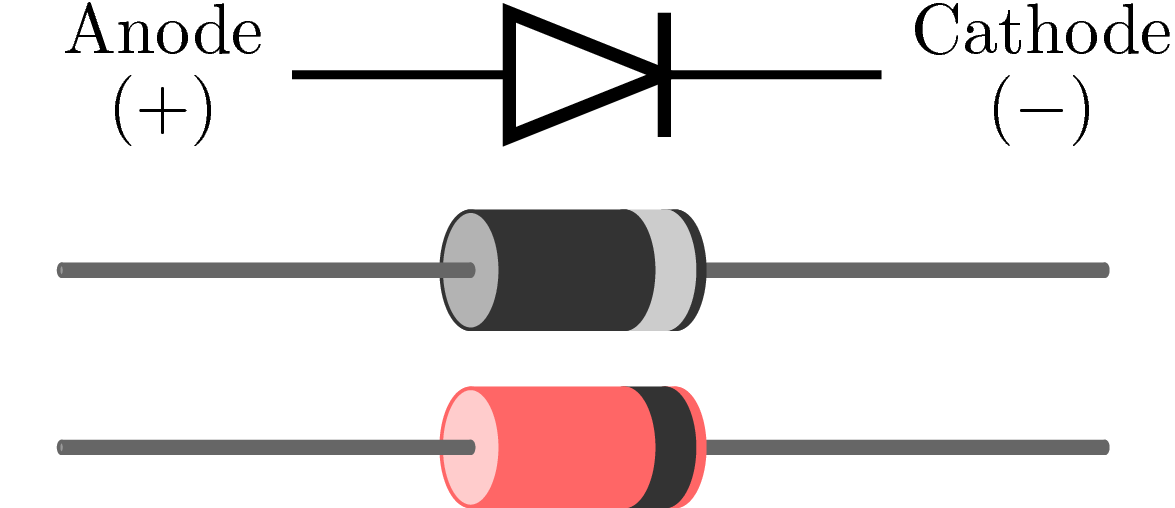
\includegraphics[width=0.5\textwidth]{./img/dioder}

\subsubsection{Ideell karakteristikk og Bulk resistance}
Ideelt sett skulle en diode blokkere strøm i en retning,
og slippe igjennom \emph{all} strøm i motsatt retning.
\\\\
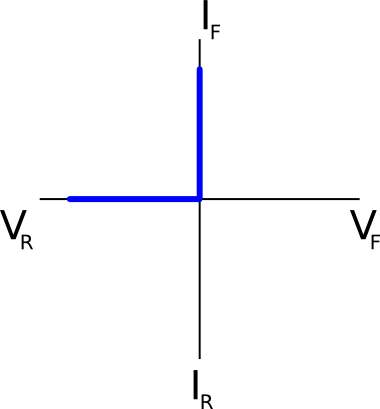
\includegraphics[width=0.5\textwidth]{./img/diodestrom}
\\\\
I virkeligheten er det en naturlig motstand
(bulk resistance) i envher diode.
\\\\
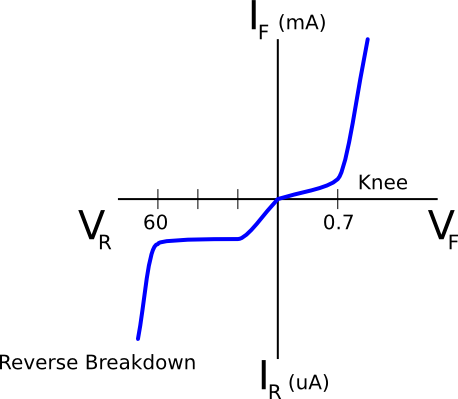
\includegraphics[width=0.5\textwidth]{./img/diodereell}

\subsubsection{Temperatureffekt}
TODO

\subsubsection{Eksempel}
Finn strømmen!\\
(Husk at dioder har en potensialbarriere på ca 0.7 Volt)
\\\\
$V_S = \SI{5}{\volt} \quad
 R = \SI{1}{k\ohm}$
\\\\
\begin{circuitikz} \draw
(0,0) node[ground]{}
      to[battery, label=$V_S$] (0,3)
      to[R, label=$R$] (3,3)
      to[diode, label=$D$] (3,0)
      node[ground]{}
      ;
\end{circuitikz}

Etter Kirchhoffs lov om spenninger vet vi at
$$V_S = V_R + V_D$$
Videre ser vi at
$$V_R = V_S - V_D = 5 - 0.7 = \SI{4.3}{\volt}$$
Strømmen er gitt ved
$$I_R = \frac{V_R}{R} = \frac{4.3}{1\cdot 10^3} = \SI{4.3}{m\ampere}$$


\subsubsection{Ulike typer dioder}
\paragraph{Zenerdioder} \mbox{} \\
Zenerdioder viker i \emph{Reverse Breakdow} området i diodens virkeområde.
Det vil si, når spenningen er revers i forhold til diodens retning.
\\
De brukes som bl.a. spenningsregulator fordi
stor forandring i strøm fører til liten forandring i spenning.

\paragraph{Varicap} \mbox{} \\
Varicapdiode, variable capacitance diode,
brukes som en variabel kondensator.
Kan brukes i radioaparater for å stille inn ønsket frekvens.

